\documentclass[12pt,a4paper]{article}
\usepackage[utf8]{inputenc}
\usepackage{amsmath}
\usepackage{amsfonts}
\usepackage{amssymb}
\usepackage{listings}
\usepackage{url}
\usepackage[bulgarian]{babel}
\usepackage{listings}
\usepackage{enumerate}
\usepackage[framemethod=tikz]{mdframed}
\usepackage{enumitem}
\usepackage{relsize}
\usepackage{hyperref}
\usepackage{caption}
\usepackage{tikz}
\usetikzlibrary{shapes,arrows,positioning,calc,chains}

\captionsetup{font=footnotesize}

\lstset{breaklines=true}

\setenumerate[1]{label=\thesection.\arabic*.}
\setenumerate[2]{label*=\arabic*.}

\newcommand{\code}[1]{\texttt{#1}}

\hypersetup{
    colorlinks,
    citecolor=black,
    filecolor=black,
    linkcolor=black,
    urlcolor=black
}

\tikzset{
block/.style = {draw, fill=white, rectangle,align = center},
entry/.style = {draw, fill=black, circle, radius=3em},
condition/.style = {draw, fill=white, diamond, align = center,node distance=3cm},
fork/.style = {draw, fill=black, circle,inner sep=1pt},
lnode/.style={rectangle split, rectangle split parts=3,draw, rectangle split horizontal}
}


\author{\textit{email: kalin@fmi.uni-sofia.bg}}
\title{\textsc{Задачи за задължителна самоподготовка} \\
по \\
Структури от данни в програмирането}


\begin{document}
\maketitle

\tableofcontents

\pagebreak

\section {Линеен едносвързан и двусвързан списък}

\subsection {Представяне на двусвързан списък}

\begin{mdframed}[hidealllines=true,backgroundcolor=gray!20]
Възел на линеен двусвързан списък представяме със следния шаблон на структура:
\begin{verbatim}
template <class T>
struct dllnode
{
  T data;
  dllnode<T> *next, *previous;
};
\end{verbatim}
Освен ако не е указано друго, задачите по-долу да се решат като се реализират методи на клас \code{DLList} със следния скелет:
\begin{verbatim}
template <class T>
class DLList
{
  //...
  private:
  dllnode<T> *first, *last;
};
\end{verbatim}
Преди да пристъпите към задачите, реализирайте подходящи контруктори, деструктор и оператор за присвояване на класа.
\end{mdframed}

Следните задачи да се решат като упражнение за директно боравене с възлите на линеен двусвързан списък. Функциите (методите) да се тестват с подходящи тестове.

\begin{enumerate}[resume]

	\item  Да се дефинира функция \code{int count(dllnode<T>* l,int x)}, която преброява колко пъти елементът \code{x} се среща в списъка с първи елемент \code{l}.
	\item  Фунцкция \code{dllnode<int>* range (int x, int y)} която създава и връща първия елемент на списък с елементи $x, x+1, ..., y$, при положение, че $x \leq y$.
	\item  Да се дефинира функция \code{removeAll (dllnode<T>*\& l,const T\& x)}, която изтрива всички срещания на елемента \code{x} от списъка \code{l}.
	\item  Да се дефинира функция \code{void append(dllnode*<T>\& l1, dllnode<T>* l2)}, която добавя към края на списъка $l_1$ всички елементи на списъка $l_2$. Да се реализира съответен оператор \texttt{+=} в класа на списъка.
	\item  Да се дефинира функция \code{dllnode* concat(dllnode<T>* l1, dllnode<T>* l2)}, който съединява два списъка в нов, трети списък. Т.е. \code{concat($l_1,l_2$)} създава и връща нов списък от елементите на \code{$l_1$}, следвани от елементите на \code{$l_2$}. Да се реализира съответен оператор \texttt{+} в класа на списъка.
	\item  Да се дефинира функция \code{reverse}, която обръща реда на елементите на списък. Например, списъкът с елементи $1,2,3$ ще се преобразува до списъка с елементи $3,2,1$.
	\item Да се напише функция \code{void removeduplicates (dllnode *\&l)}, която изтрива всички дублиращи се елементи от списъка $l$.
\end{enumerate}

\subsection {Списъци и сложности}
\label{timing}
\begin{mdframed}[hidealllines=true,backgroundcolor=gray!20]
Функцията \code{std::clock()} от \code{<ctime>} връща в абстрактни единици времето, което е изминало от началото на изпълнение на програмата. Обикновено тази единица за време, наречена ``\code{tick}'', е фиксиран интервал ``реално'' време, който зависи от хардуера на системата и конфирграцията ѝ. Константата \code{CLOCKS\_PER\_SEC} дава броя \code{tick}-ове, които се съдържат в една секунда реално време.

Чрез следния примерен код може да се измери в милисекунди времето за изпълнение на програмния блок, обозначен с ``...''.
\begin{verbatim}
clock_t start = std::clock();
//...
clock_t end = std::clock();

long milliseconds = (double)(end-start)/
                    (CLOCKS_PER_SEC/1000.0);

\end{verbatim}
\end{mdframed}

\begin{enumerate}[resume]

\item За шаблона DLList да се дефинира метод \texttt{bool find(const T\& x)}, който проверява дали дали \texttt{x} е елемент на списъка или не. Да се напише подходящ тест и да се изследва времевата сложност на метода емпирично.

\item За шаблона \texttt{DLList} да се реалзиира изтриване на елемент по индекс.

\item Да се изпробват поне две различни стратегии за разширяване на динамичен масив (например, увеличаване на размера с 1 и с коефициент). Да напишат подходящи тестове и да се сравнят производителностите на двата подхода емпирично.

\end{enumerate}

\subsection {Итератори за линейни СД}
\label{iterators1}
Следните задачи да се решат като упражнение за работа с итератори. Задачите изискват реализация на клас динамичен масив и линеен двусвързан списък и \code{forward} итератори за тях. Всяка функциия да се тества с подходящи тестове върху двата вида контейнери. Има ли разлика в проиводителността за някои от тях в зависимост от избора на контейнер?


\begin{enumerate}[resume]

	\item Да се разшири интераторът на динамичен масив така, че да поддържа оператора за стъпка назад \texttt{-{}-}.

	\item  Да се дефинира функция \code{map}, която прилага едноаргументна функция $f:int \rightarrow int$ към всеки от елементите на произволен контейнер. Да се дефнира и шаблон на функцията за списък с произолен тип на елементите.

	\item Да се напише функция \code{bool duplicates (...)}, която проверява дали в контейнер има дублиращи се елементи.

	\item Да се напише фунцкия \code{bool issorted (...)}, която проверява дали елементите на даден контейнер са подредени в нарастващ или в намаляващ ред.

	\item Да се напише фунцкия \code{bool palindrom (...)}, която проверява дали редицата от елементите на даден контейнер обрзува палиндром (т.е. дали се чете еднакво както отляво надясно така и отдяно наляво).

\end{enumerate}


\subsection{Skip List}


\begin{mdframed}[hidealllines=true,backgroundcolor=gray!20]
Разглеждаме \emph{опростена} реализация на структурата от данни Skip List (``Списък с прескачене, СП''). Възелът на линейния едносвързан списък разширяваме с още един указател към следващ елемент:

\begin{verbatim}
template <class T>
struct lnode
{
  T data;
  lnode<T> *next[2];
};
\end{verbatim}
Както и при стандартния едносвързан списък, всеки от елментите на СП съдържа в указателя \code{next[0]} адреса на непосредствения си съсед. Някои от елементите могат да съдържат в указателя \code{next[1]} дреса на друг елемент, намиращ се по-напред в редицата от елементи (вж. Фигура \ref{fig:skiplist}). Например, нека имаме СП с $n$ елемента в нарастващ ред. Ако списъкът е построен така, че всеки $\sqrt{n}$-ти елемент има указател към следващия  $\sqrt{n}$-ти елемент, то търсенето на елемент ще бъде със сложност $O(\sqrt{n})$ на цената на линейно нарастване на необходимата памет. Идеята може да се продължи така, че всеки елемент да може да има и по-голям брой указатели към елементи все по-напред в СП, но за нашите цели ще се ограничим до описания прост СП.

Следващите задачи изискват реализация на клас \code{SkipList} с основните му канонични методи и метод за построяване на ``бързите връзки''. Реализирайте обиновен метод за вмъкване на елементи \code{insert}, който вмъква елементи грижейки се само за непосредствените връзки (\code{next[0]}), и метод \code{optimize}, който построява бързите връзки в списъка след като в него са вмъкнати определен брой елементи.
\end{mdframed}

\begin{figure}
  \centering

    \begin{tikzpicture}[auto, node distance=2cm,>=latex']
    \node[lnode] (n1) {\nodepart{two}1};
    \node[lnode, right of = n1] (n2) {\nodepart{two}2};
    \node[lnode, right of = n2] (n3) {\nodepart{two}3};
    \node[lnode, right of = n3] (n4) {\nodepart{two}4};
    \node[lnode, right of = n4] (n5) {\nodepart{two}5};

    \node[rectangle,left of = n1](start){};

    \draw[*->]  (start)-- (n1);

    \draw[*->] let \p1 = (n2.three), \p2 = (n1.center) in (\x1,\y2) -- (n3);
    \draw[*->] let \p1 = (n1.three), \p2 = (n1.center) in (\x1,\y2) -- (n2);
    \draw[*->] let \p1 = (n3.three), \p2 = (n1.center) in (\x1,\y2) -- (n4);
    \draw[*->] let \p1 = (n4.three), \p2 = (n1.center) in (\x1,\y2) -- (n5);
    \draw[*->,dashed] let \p1 = (n1.one), \p2 = (n1.center) in ([shift={(0.1cm,-0.1cm)}]\x1,\y2) |-([shift={(0,0.5cm)}]n1.north east) -- ([shift={(0,0.5cm)}]n3.north) -| (n3);
    \draw[*->,dashed] let \p1 = (n3.one), \p2 = (n3.center) in ([shift={(0.1cm,0.1cm)}]\x1,\y2) |-([shift={(0,-0.5cm)}]n3.south east) -- ([shift={(0,-0.5cm)}]n5.south) -| (n5);
    \end{tikzpicture}
  \caption{Списък с прескачане}
  \label{fig:skiplist}
\end{figure}

\begin{enumerate}[resume]


  \item  Да се реализира итератор на \code{SkipList} така, че да се възползва от ``бързите връзки'' в списъка. \textit {Упътване: при обхождането извършвайте ``прескачане'' в случаите, в които има бърза връзка и в които няма да отидете твърде далеч напред в списъка. Класът на итератора трябва да се промени, за да позволява конструиране на итератор към конкретен елемент на списъка}.
	\item  Да се извърши времево измерване на проблема за търсене на елемент в подреден \code{SkipList}, както е обяснено в Секция \ref{timing}, и да се изобрази чрез графика. Да се извършат емпирични сравнения на производителността на търсенете със и без оптимизацията.

\end{enumerate}


\pagebreak

\section {Двоични дървета}
\begin{mdframed}[hidealllines=true,backgroundcolor=gray!20]
Възел на двоично дърво представяме със следния шаблон на структура:
\begin{verbatim}
template <class T>
struct btreenode
{
  T data;
  btreenode<T> *left, *right;
};
\end{verbatim}
Освен ако не е указано друго, задачите по-долу да се решат като се реализират методи на клас \code{BTree} със следния скелет:
\begin{verbatim}
template <class T>
class BTree
{
  //...
  private:
  btreenode<T> *root;
};
\end{verbatim}
Преди да пристъпите към задачите, реализирайте подходящи контруктори, деструктор и оператор за присвояване на класа.
\end{mdframed}

\begin{enumerate}[resume]

	\item Да се деифнира метод \texttt{count} на клас \texttt{BTree}, който намира броя на елементите на дървото.

	\item Да се деифнира метод \texttt{countEvens} на клас \texttt{BTree}, който намира броя на елементите на дърво от числа, които са четни.


	\item Да се дефинира метод \texttt{int BTree<T>::searchCount (bool (*pred)(const T\&))} към клас \texttt{BTree}, който намира броя на елементите на дървото, които удовлетворяват предиката \texttt{pred}.

	Да се приложи \texttt{searchCount} за решаване на горните две задачи.

	\item Да се дефинира метод \texttt{bool BTree<T>::height ()}, намиращ височината на дърво. \textit{Височина на дърво наричаме дължината (в брой върхове) на най-дългия път от корена до кое да е листо на дървото.}
	\textit{Пример. Височината на дървото на Фигура \ref{fig:tree1} е \textbf{3}.}

  \begin{figure}
  \centering
	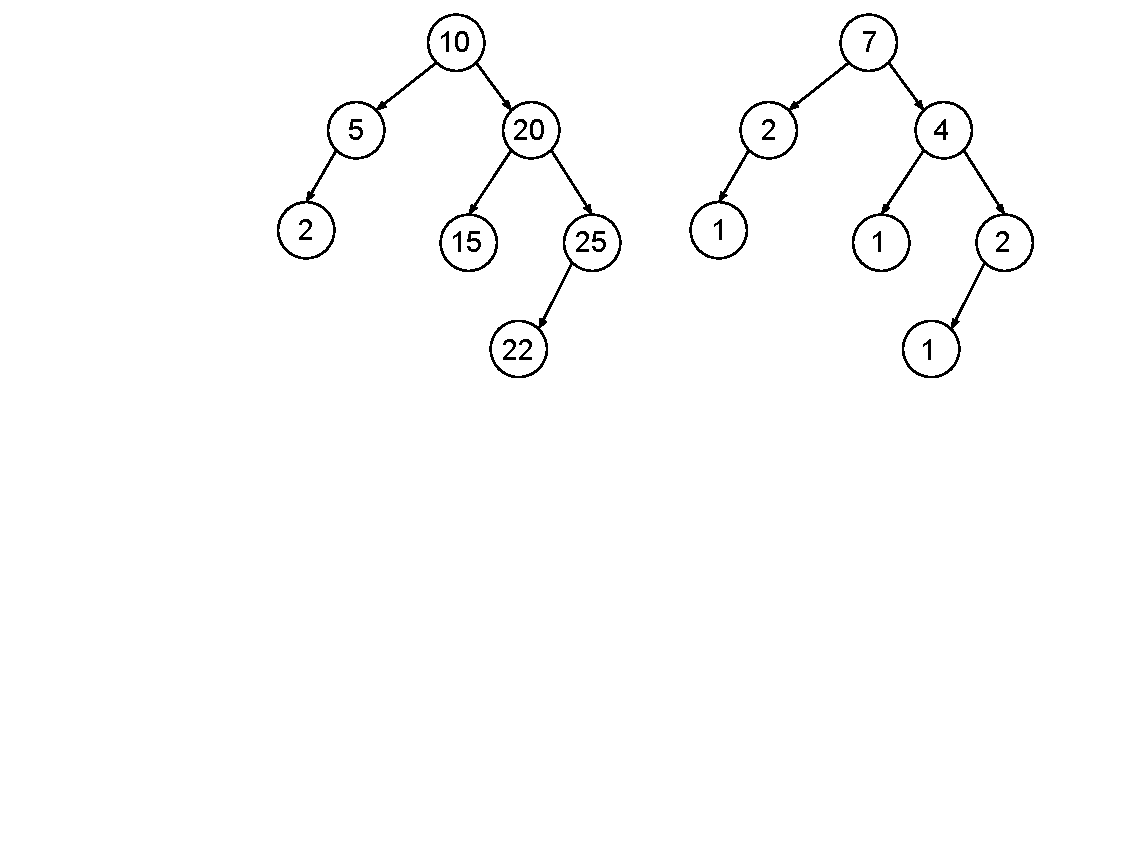
\includegraphics[width=4cm]{images/tree1}

	\caption{Двоично наредено дърво}
  \label{fig:tree1}
  \end{figure}


	\item Да се деифнира метод \texttt{countLeaves} на клас \texttt{BTree}, който намира броя на листата в дървото.

	\item Да се деифнира метод \texttt{maxLeaf} на клас \texttt{BTree}, който намира най-голямото по стойност листо на непразно дърво. Да се приеме, че за типа \texttt{T} на шаблона \texttt{BTree} е дефиниран операторът \texttt{<}.

	\item Нека е дадено дървото \texttt{t} и низът \texttt{s}, съставен само от символите `L' и `R' ($s \in \{L,R\}^*$). Нека дефинираме ``съответен елемент'' на низа \texttt{s} в дървото \texttt{t} по следния начин:
	\begin{itemize}
		\item Ако дървото \texttt{t} е празно, низът \texttt{s} няма съответен елемент
		\item Ако низът \texttt{s} е празен, а дървото \texttt{t} - не, то коренът на дървото \texttt{t} е съответният елемент на низа \texttt{s}
		\item Ако първият символ на низа \texttt{s} е `L' и дървото \texttt{t} не е празно, то съответният елемент на низа \texttt{s} в дървото \texttt{t} е съответният елемент на низа $s+1$ в \textbf{лявото} поддърво на \texttt{t}
		\item Ако първият символ на низа \texttt{s} е `R' и дървото \texttt{t} не е празно, то съответният елемент на низа \texttt{s} в дървото \texttt{t} е съответният елемент на низа $s+1$ в \textbf{дясното} поддърво на \texttt{t}
	\end{itemize}

	\textit{Пример. За 	дървото от Фигура \ref{fig:tree1}, съответният елемент на празния низ е 10, на низа ``RL'' е 15, а ``RLR'' няма съответен елемент.}

	Да се дефинира метод \texttt{T\& BTree<T>::getElement (const char *s)}, който намира съответния елемент на низа \texttt{s}. Какво връща методът в случаите на липса на съответен елемент е без значение.


\end{enumerate}





\pagebreak

\begin{thebibliography}{99}

%\bibitem{sbornik}	Магдалина Тодорова, Петър Армянов, Дафина Петкова, Калин Георгиев, ``Сборник от задачи по програмиране на C++. Първа част. Увод в програмирането''

\end{thebibliography}

\end{document}
